\documentclass[tikz]{standalone}
\usepackage{pgfplots}
\pgfplotsset{compat=1.18}

\begin{document}
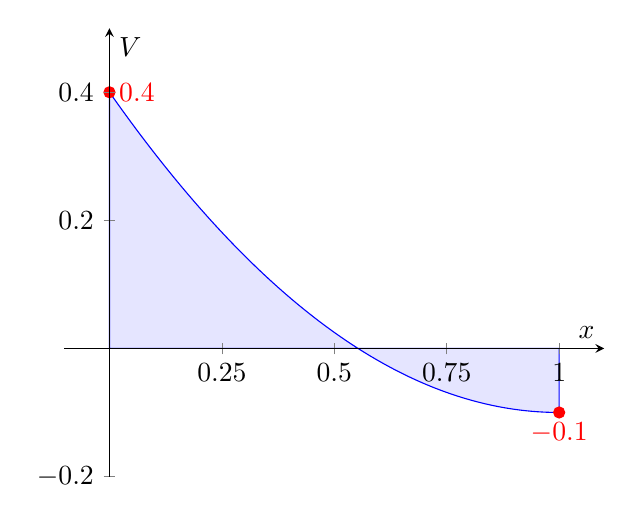
\begin{tikzpicture}
	\begin{axis}[
		axis lines = middle,
		xlabel = $x$,
		ylabel = {$V$},
		xmin=-.1, xmax=1.1,
		ymin=-.2, ymax=0.5,
		xtick={0, 0.25, 0.50, 0.75, 1},
		set layers, % Activa las capas
		axis on top % <-- Agrega esta opción
		]
		\addplot [
		domain=0:1, 
		samples=100, 
		color=blue,
		fill=blue!10,
		]
		{2/5 - x + 0.5*x^2} \closedcycle;
		
		% Punto máximo
		\addplot[mark=*, color=red] coordinates {(0,0.4)} node[right] {$0.4$};
		
		% Punto mínimo
		\addplot[mark=*, color=red] coordinates {(1,-0.1)} node[below] {$-0.1$}; 
	\end{axis}
\end{tikzpicture}
\end{document}